\setchapterstyle{kao}
\setchapterpreamble[u]{\margintoc}

\todo{increase main text width (read in kao docu)}


\chapter{Standard Model Background Simulation and Data Processing}
\labch{simulation_and_processing}

The analysis presented in this thesis is highly dependent on an efficient event selection to reduce the raw IceCube trigger data to a usable atmospheric neutrino sample. Based on this selection a precise estimation of both expected SM background and expected BSM signal events can be made using MC simulations. This chapter describes the current simulation and event selection chain used for state-of-the-art IceCube neutrino oscillation measurements like \sidecite[0.3cm]{OVS_PRD}. The whole chain can be broadly split into 4 steps:

\begin{enumerate}[wide]
    
    \item[]{\textbf{Step 1 Event Generation:}} The initial step for all particle (non-noise) simulation is the generation of events from selected initial distributions and fluxes. Events are the primary particle and the particles produced in the interaction with the ice.
    \vspace{0.2cm} 

    \item[]{\textbf{Step 2 Detector Simulation:}} The particles from the first step are propagated through the ice, producing Cherenkov photons, which are then propagated further until they reach a DOM or are absorbed. If they hit a DOM the detector response (acceptance and PMT) is simulated.
    \vspace{0.2cm} 
        
    \item[]{\textbf{Step 3 Processing:}} Starting from the PMT output, both real data and simulation are processed through the in-ice trigger, the online filter and processing, and the low energy event selection to produce a neutrino dominated sample.
    \vspace{0.2cm} 

    \item[]{\textbf{Step 4 Reconstruction:}} Once the sample is small enough for more sophisticated reconstruction techniques to be feasible to run, the events are reconstructed using a CNN and some high level variables are computed. Based on these variables the final event selection is applied.
    
\end{enumerate}

This chapter only describes the event generation for the SM background simulation (neutrinos and muons), while the signal simulation is described in \refch{signal_simulation}. The detector simulation is identical for both signal and background events while processing and reconstruction are applied to all simulation and data in the same way. Splitting the simulation steps has the advantage of reusing the outputs of for example the generation step to propagate the particles with different ice model, in order to estimate the systematic impacts of uncertainties of the ice properties. Similar approach can be taken for varying detector response and through this a more efficient (reduced) use of computing resources can be achieved. The following sections describe the different steps in more detail and the last section, \refsec{systematic_uncertainties}, describes the related systematic uncertainties considered for this work.


\section{Event Generation} \labch{sm_event_generation}

The MC is used in the analysis by applying a method called \textit{forward folding}, where a very large number of events (signal and background) is produced using sampling distribution that are tuned to have a large selection efficiency. Those distributions don't have to be physically correct distributions, but they need to cover the full parameter space of interest for the analysis. To produce the correct physical distributions each event gets a weight, which can be used to estimate the expected number of events given a specific choice of physics and nuisance parameters. The large number of raw MC events ensures a good estimation of the expected numbers and weighted distributions. 

The analysis itself is then performed by comparing the weighted MC distributions to the observed data. This is done by binning them as will be described in \refch{analysis} and calculating a loss function comparing the bin expectations to the data. By varying the physics and nuisance parameters, that govern the weights, the loss function can be minimized and the parameters producing MC that describes the data best are found. In order to achieve a reliable result with this method the MC needs to be precise and as close to the data as possible (at least at the final selection step). 


\subsection{Neutrinos}

Due to the very low interaction rate of neutrinos, the event generation is performed in a way that forces every event to interact in a chosen sampling volume. The weight of each event is then calculated as the inverse of the simulated neutrino fluence
\begin{equation}
    w = \frac{1}{F_{\mathrm{sim}}} \frac{1}{N_{\mathrm{sim}}}
    \;,
    \labeq{neutrino_generation_weight}
\end{equation}
where $F_{\rm{sim}}$ is the number of neutrino events per energy, time, area, and solid angle and $N_{\rm{sim}}$ is the number of simulated events. If this weight is multiplied by the livetime and the theoretically expected neutrino flux for a given physical model, it results in the number of events that this event would produce. The used baseline neutrino flux computed for the South Pole is taken from Honda \textit{et al.} \sidecite{PhysRevD.92.023004_Honda_Flux}.

The chosen simulation volume is a cylinder centered in DeepCore with radius and height chosen such that all events possibly producing a signal are contained. The different sizes are chosen depending on energy and neutrino flavor are shown in \reftab{genie_sampling_cylinder}.
\begin{table}
    \begin{center}
        % \small
        \footnotesize
        % \begin{tabular}{ p{1.0cm} p{1.8cm} p{1.3cm} p{1.3cm} p{1.4cm} p{0.6cm} }
        \begin{tabular}{ l l l l l l }

            \hline\hline

            \textbf{Flavor} & \textbf{Energy [\si{\gev}]} & \textbf{Radius [\si{\metre}]} & \textbf{Length [\si{\metre}]} & \textbf{Events/File}  & \textbf{Files}\\ 

            \hline\hline

            \multirow{4}{*}[-1.em]{ $\nu_e+\bar{\nu_e}$ }
            & 1-4
            & \multirow{1}{*}[-1.em]{ 250 }
            & \multirow{1}{*}[-1.em]{ 500 }
            & 450000
            & \multirow{4}{*}[-1.em] {650} \\

            \cmidrule{2-2}
            \cmidrule{5-5}
            
            & 4-12
            & 
            & 
            & \multirow{1}{*}[-1.em] { 100000 }
            & \\

            \cmidrule{2-4}

            & 12-100
            & 350
            & 600
            & 
            & \\

            \cmidrule{2-5}

            & 100-10000
            & 550
            & 1000
            & 57500
            & \\

            \hline
            \hline

            \multirow{4}{*}[-1.em]{ $\nu_\mu+\bar{\nu_\mu}$ }
            & 1-5
            & 250
            & 500
            & 408000
            & \multirow{4}{*}[-1.em] {1550} \\

            \cmidrule{2-5}
            
            & 5-80
            & 400
            & 900
            & 440000
            & \\

            \cmidrule{2-5}

            & 80-1000
            & 450
            & \multirow{1}{*}[-1.em] { 1500 }
            & 57500
            & \\

            \cmidrule{2-3}
            \cmidrule{5-5}

            & 1000-10000
            & 550
            &
            & 6700
            & \\

            \hline
            \hline

            \multirow{4}{*}[-1.em]{ $\nu_\tau+\bar{\nu_\tau}$ }
            & 1-4
            & \multirow{1}{*}[-1.em]{ 250 }
            & \multirow{1}{*}[-1.em]{ 500 }
            & 1500000
            & \multirow{4}{*}[-1.75em] {350} \\

            \cmidrule{2-2}
            \cmidrule{5-5}
            
            & 4-10
            & 
            & 
            & 300000
            & \\

            \cmidrule{2-5}

            & 10-50
            & 350
            & 600
            & 375000
            & \\

            \cmidrule{2-5}

            & 50-1000
            & 450
            & 800
            & 200000
            & \\

            \cmidrule{2-5}

            & 1000-10000
            & 550
            & 1500
            & 26000
            & \\

            \hline

        \end{tabular}
    \end{center}
    \caption[GENIE generation cylinder volumes]{Cylinder volumes used for GENIE neutrino simulation generation. Cylinder is always centered in DeepCore at $(x,y,z) = (46.29,-34.88,-330.00)$ \si{\metre}.}\labtab{genie_sampling_cylinder}
\end{table}
The directions of the neutrinos are sampled isotropically in zenith and azimuth and the energies are sampled from a power law $E^{-2}$. The number of simulated events is chosen such that the livetime is more than \SI{70}{years} for each flavor. Neutrinos and antineutrinos are simulated with ratios of 70\% and 30\%, respectively.

To simulate the neutrino interaction with the ice the \textsc{Genie} event generator \sidecite{genie} is used, resulting in the secondary particles and the kinematic and cross-section parameters. As input, the outdated GRV98 \sidecite{grv98_pdf} \textit{parton distribution functions (PDFs)} was used, because it was the only option that could incorporate extrapolations to lower $Q^2$ \sidecite{grv98_effective_low_q2}. Muons produced in these interactions are propagated using \textsc{Proposal} \sidecite{proposal}, also simulating their Cherenkov light output. The shower development of gamma rays, electrons, and positrons below \SI{100}{\mega\electronvolt} and hadronic showers below \SI{30}{\gev} is simulated using \textsc{Geant4} \sidecite{geant4} while for higher energies an analytical approximation from \sidecite{raedel_wiebusch_cherenkov_yield} is used.


\subsection{Muons}

Atmospheric muons are generated on a cylinder surface enclosing the full IceCube detector array. The cylinder has a height of \SI{1600}{\meter} and a radius of \SI{800}{\meter}. The energy is sampled from an $E^{-3}$ power law while the other sampling distributions (position, direction) are found from parameterizations based on \sidecite{muon_parameterization}. This work uses full \textsc{Corsika} \sidecite{corsika} simulations of muons to tailor the parameterizations, starting from cosmic ray interactions with atmospheric nuclei using the cosmic ray flux model from \sidecite{gaisser_cosmic_ray} and producing the muons applying the hadronic interaction model SIBYLL 2.1 \sidecite{sibyll_hadronic}. After the generation, they are propagated through the ice with PROPOSAL producing photons, treating them exactly like the muons produced in neutrino interactions.

Since the offline processing and selection steps described in \refsec{offline_filter} and \refsec{reconstruction} reduce the muon contamination to a negligible level, it is difficult to correctly estimate the expected number of muon events at final selection level and therefore two separate sets of muon simulation are produced. \textbf{A first set} including all events resulting from the above described generation to tune the lower level selection (up to L4) and \textbf{a second set} to estimate the muon contamination at higher levels (above L5), which only accepts muon events if they pass through a smaller cylinder centered in DeepCore (height of \SI{400}{\meter} and radius of \SI{180}{\meter}) and rejects events based on a KDE estimated muon density at L5 (in energy and zenith) increasing the simulation efficiency at L5 significantly \todo{put a number on this significant increase?}.


\section{Detector Simulation}

The detector simulation is performed after the event generation, where the initial particles and the resulting photons and secondary particles from their propagation were produced. This part of the simulation chain is applied to all particle simulation, both neutrino and muon generation explained in \refch{sm_event_generation}, but also the particles from the HNL signal generation explained in detail in \refch{signal_simulation}. The detector simulation can be split into two parts, the propagation of the photons and the simulation of the detector response (including internal noise).


\subsection{Photon Propagation}

For any Cherenkov detector, but especially for ice-Cherenkov detectors, like IceCube, the propagation of the photons is a crucial part of the detector simulation. Any photon that was produced in the event generation is individually traced through the ice, simulating scattering and absorption processes, taking into account the local ice properties, estimated with a chosen ice model. The propagation is done using \textsc{clsim} \cite{clsim} which is an implementation of the \textit{Photon Propagation Code (\textsc{PPC})} \sidecite{ppc} in \textsc{OpenCL}. It is optimized to be run very efficiently on GPUs, which is what is done for IceCube simulation production. The ice is modeled as a set of \SI{10}{\meter} thick, almost horizontal layers with specific absorption and scattering lengths. The \textit{South Pole ice (SPICE)} model \sidecite{spice_ice_model} accounts for the layers being tilted by a small amount (\todo{put a number on the tilt angle?}) and the absorption and scattering lengths having a non-uniformity with respect to the azimuth direction. \reffig{simulation_ice_model} shows the values of this model for the different depths, indicating the location of IceCube, DeepCore, and the dust layer.

\begin{figure}
    \begin{tikzpicture}
\pgfplotsset{set layers}

\pgfplotstableread{figures/icecube_deepcore/spice/icemodel.dat}\table

\begin{axis}[
    tab_blue,
    y axis line style={black},
    scale only axis,
    width=0.7\linewidth,
    height=0.5\linewidth,
    xmin=1100,xmax=2900,
    xticklabel style={/pgf/number format/.cd,1000 sep={}},
    axis y line*=left, % the '*' avoids arrow heads
    axis x line=none,
    ymin=0,
    enlarge y limits=true,
    xlabel=depth {[m]},
    ylabel=scattering length {[m]},
]

    \addplot[tab_blue, thick] table [x index=0, y expr=1 / \thisrowno{1}] \table;

    % dust layer
    \draw [name path=dust layer top, gray, thin] (1970, \pgfkeysvalueof{/pgfplots/ymin}) -- (1970, \pgfkeysvalueof{/pgfplots/ymax});
    \draw [name path=dust layer bottom, gray, thin] (2080, \pgfkeysvalueof{/pgfplots/ymin}) -- node[near end, sloped, above, black, font=\footnotesize\sffamily] {dust layer} (2080, \pgfkeysvalueof{/pgfplots/ymax});
    \addplot [gray, opacity=0.4] fill between [of=dust layer top and dust layer bottom];

    % IceCube
    \draw [name path=icecube top, gray, thin] (1450, \pgfkeysvalueof{/pgfplots/ymin}) -- (1450, \pgfkeysvalueof{/pgfplots/ymax});
    \draw [name path=icecube bottom, gray, thin] (1970, \pgfkeysvalueof{/pgfplots/ymin}) -- (1970, \pgfkeysvalueof{/pgfplots/ymax});
    \node[anchor=south, black, font=\footnotesize\sffamily] at (1750, 110) {IceCube\strut};
    \addplot [gray, opacity=0.2] fill between [of=icecube top and icecube bottom];

    % DeepCore
    \draw [name path=deepcore top, gray, thin] (2080, \pgfkeysvalueof{/pgfplots/ymin}) -- (2080, \pgfkeysvalueof{/pgfplots/ymax});
    \draw [name path=deepcore bottom, gray, thin] (2450, \pgfkeysvalueof{/pgfplots/ymin}) -- (2450, \pgfkeysvalueof{/pgfplots/ymax});
    \node[anchor=south, black, font=\footnotesize\sffamily] at (2270, 110) {DeepCore\strut};
    \addplot [gray, opacity=0.1] fill between [of=deepcore top and deepcore bottom];

\end{axis}

\begin{axis}[
    tab_orange,
    scale only axis,
    width=0.7\linewidth,
    height=0.5\linewidth,
    xmin=1100,xmax=2900,
    axis y line*=right,
    axis x line=none,
    ymin=0,
    enlarge y limits=true,
    ylabel=absorption length {[m]},
]

    \addplot[tab_orange, thick] table [x index=0, y expr=1 / \thisrowno{2}] \table;

\end{axis}

\begin{axis}[
    scale only axis,
    width=0.7\linewidth,
    height=0.5\linewidth,
    xmin=1100,xmax=2900,
    xticklabel style={/pgf/number format/.cd,1000 sep={}},
    axis y line*=left, % the '*' avoids arrow heads
    xlabel=depth {[m]},
    axis y line=none,
]

\addplot[tab_orange, thick] table [x index=0, y expr=1 / \thisrowno{2}] \table;


\end{axis}

\end{tikzpicture}

	\caption[Depth dependent scattering and absorption lengths]{Scattering and absorption lengths in the SPICE model used for simulation production as a function of depth, modified from \cite{ATrettin_phd}.}
    \labfig{simulation_ice_model}
\end{figure}

In an initial step, each photon's absorption length is sampled from an exponential distribution with the expectation value at the current layer's absorption length. The following propagation steps are performed in parallel for all photons. In each of those steps, corresponding to a single scattering event, the photon travels a length that is sampled from an exponential distribution with the expectation value at the scattering length of the current layer and the scattering angle chosen based on a combination of a simplified Mie scattering distribution \sidecite{mie_scattering} and a Henyey-Greenstein distribution \sidecite{henyey_greenstein}. The parameters defining the shape of these distributions were calibrated using data from \textit{in-situ} LED calibration runs. These steps are continuously repeated until each photon reached a DOM or was absorbed\sidenote{A photon is absorbed, when it traveled its full absorption length, sampled in the initial step of the photon propagation.}. After all photons have been propagated in that manner, the final step is to output the photons that reached a DOM for further processing.


\subsection{Detector Responses}

The second part of simulating the IceCube detector is the DOM response itself, but not all the photons that reached a DOM are accepted as being observed. Whether a photon was detected is determined individually based on the total efficiency and the angular acceptance curve of the specific DOM. The total efficiency includes effects of the DOM glass, PMT quantum and photo-electron collection efficiencies, and it is wavelength dependent. Additionally, there is another angle dependent effect called \textit{hole ice}. This effect is due to varied ice properties resulting from the re-freezing process of the water column inside the borehole after deployment of the string. Due to bubble formation the ice is less transparent than the surrounding ice and an additional angular acceptance is added, which can increase or decrease the efficiency to detect photons. Accepted photons are converted into a so-called \textit{Monte Carlo photo-electron (MCPE)}. The amount of charge measured for each MCPE is determined by sampling from a mixture of two exponential distributions and a normal distribution. This \textit{single photo-electron (SPE)} distribution was tuned to match the observed distribution in each DOM in an \textit{in-situ} calibration study \sidecite{spe_respose_pmt}. \reffig{spe_distribution} shows the distribution compared to a lab measurement. Based on the sampled charges and times of MCPEs, the voltage waveforms for the (two) different readout channels are simulated and passed on to the trigger simulation starting with \textit{WaveDeform}, which was already mentioned in \refsec{ice_and_DOMs}.

\begin{margintable}
\small
    % \begin{tabular}{ p{0.48\textwidth} p{0.35\textwidth} }
    \begin{tabular}{ ll }
    \hline\hline

    \textbf{Parameter} & \textbf{Value} \\ 

    \hline\hline

    Therm. rate $\lambda_\mathrm{th}$ & $\SI{180}{\hertz}$ \\
    Decay rate $\lambda_\mathrm{dec}$ & $\SI{80}{\hertz}$ \\
    Decay hits $\eta$ &  $8.5$ \\
    Decay $\mu$ & 4.3 $\log_{10}$(\si{\nano\second}) \\
    Decay $\sigma$ & 1.8 $\log_{10}$(\si{\nano\second}) \\

    \hline
    \end{tabular}
\caption[Vuvuzela noise simulation parameters]{Typical parameter values used in the vuvuzela noise simulation. Averaged over all DOMs.}
\labtab{vuvuzela_parameters}
\end{margintable}

Next to the Cherenkov photons, IceCube also observes photons that are produced in radioactive decays inside the DOMs, both in the glass housing sphere and the PMT glass itself. To simulate this internal noise, the \emph{Vuvuzela} module \sidecite{MLarson_master, MLarson_phd} is used to create additional MCPEs that are fed into the same simulation chain described above. This module takes into account thermal and non-thermal components and their times are sampled using parameterizations of the measured distributions, where the thermal noise component is uncorrelated photons and the non-thermal component is from burst of photons. The noise hits are simulated by drawing the times from a constant rate Poisson process and the number of photons from a Poisson distribution, then the time differences between the individual photons per hit is found, based on a Log-Normal distribution. The simulation is defined by 5 parameters that are calibrated for each DOM individually. \reftab{vuvuzela_parameters} shows a set of typical values for these parameters.


\section{Processing}

After the detector simulation is performed, all MC and data are processed in exactly the same way. This section explains the trigger and event selection that is applied starting from the raw voltage measured by the PMTs. Most parts of this processing are identical to the procedure already described in \sidecite{ATrettin_phd, ELohfink_phd}. It is split in different steps run inside the ice, at the South Pole, and after the data was transferred to the North. The complexity and computational cost of the processing increases with each step, while the total number of events reduces, making it feasible and reducing the use of computational resources on events that are not of interest for the analysis. 


\subsection{Trigger and Filter} \labsec{trigger_and_filter}

Before the data can be sent to the North, the initial signal coming from the PMT (for data) or from the detector response simulation (for MC) is a voltage waveform, which has to be digitized and information of photon hits has to be extracted. The trigger and filter explained here are tailored to select events that passed through the DeepCore volume, while rejecting background events (either from atmospheric muons or from random noise). There are other filters used in IceCube which will not be explained here, since they are not relevant for this work. A full description of the instrumentation and the online systems can be found in \sidecite{Aartsen:2016nxy}.


\subsubsection{In-ice Trigger} \labsec{trigger}

\begin{marginfigure}
    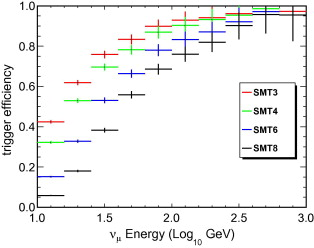
\includegraphics{figures/simulation_and_processing/trigger/trigger_efficiency.jpg}
	\caption[IceCube trigger efficiencies]{Efficiencies of different IceCube and DeepCore triggers, taken from \cite{DeepCore_design_Abbasi2012615}.}
    \labfig{trigger_efficiencies}
\end{marginfigure}

The trigger is applied inside the DOM in the ice before sending the information to the ICL on the surface. The time dependent voltage curves are captured if a pre-defined threshold value is exceeded. Once the threshold set to the equivalent of \SI{0.25}{PE} is crossed, \SI{6.4}{\micro\second} of the waveform are coarsely digitized by a \textit{Fast Analog-to-Digital Converter (FADC)} with a sampling rate of \SI{40}{\mega\hertz} \sidecite{ABBASI2009294_data_acquisition}. Additionally, the first \SI{427}{\nano\second} are digitized using an \textit{Analog Transient Waveform Recorder (ATWD)} with a sampling rate of \SI{300}{\mega\hertz} \sidecite{ABBASI2009294_data_acquisition}, but only if some trigger condition is met, because this readout frequency is too high to be sampled directly and requires some buffering. For DeepCore, the HLC condition already mentioned in \refsec{ice_and_DOMs} has to be met for three DOMs inside the fiducial volume within a time window of \SI{5}{\micro\second}. If this is the case, all waveforms that crossed the threshold within a \SI{20}{\micro\second} time window around the trigger are digitized and sent to the ICL for further processing. This trigger is called \textit{Simple Multiplicity Trigger 3 (SMT-3)}. The DOM hits that are read out in this process, but do not meet the HLC condition, are called \textit{soft local coincidence (SLC)} hits \sidecite{ABBASI2009294_data_acquisition}. The rate of the DeepCore SMT-3 trigger is $\sim$\SI{250}{\hertz} \sidecite{2017JInst..12P3012A_Instrumentation_Systems}, accepting $\sim$\SI{70}{\percent} of $\nu_\mu$-CC events at \SI{10}{\gev} and $\sim$\SI{90}{\percent} at \SI{100}{\gev} \sidecite{DeepCore_design_Abbasi2012615}. The trigger efficiencies for different SMT triggers, including the DeepCore SMT-3, are shown in \reffig{trigger_efficiencies}.


\subsubsection{Online Filter} \labsec{online_filter}

The digitized waveforms are sent to the ICL, where a further filter is applied \textit{online}\sidenote{Where \textit{online} means running on hardware at the South Pole.}. First the WaveDeform algorithm is run to extract photon arrival times and charge from the waveforms, then the DeepCore filter is applied, which is an iterative hit cleaning starting from HLC hits and removing any hits outside a \SI{125}{\meter} radius and a \SI{500}{\nano\second} time window (called \textit{radius-time cleaning (RT-cleaning)}) of the initial hit. This mainly rejects unphysical SLC hits, which are potentially caused by random noise. The following selection steps are done using the resulting cleaned pulses.

Next, an additional cut is applied to reject events that are likely to be caused by atmospheric muons. This is done by splitting the hits depending on whether they were inside the DeepCore fiducial volume or outside and then calculating the speed of each hit outside the fiducial volume towards the \textit{center of gravity {COG}} of the hits inside. If one of them has a speed close to the speed of light, the whole event is rejected, because this is a strong indication for a muon event.

As input for the further selection levels, a few event properties, like vertex position and direction, are determined using fast and simple event reconstructions. After the DeepCore online filter, the rate is about \SI{15}{\hertz}, which can be sent to the North via satellite for further processing.


\subsection{Event Selection} \labsec{event_selection}

After the data was sent to the North, the \textit{offline} filters and selection are applied to further recude reduce the background of atmospheric muons and noise. The selection is split into three levels referred to as \textit{Level 3-5 (L3-L5)}, which bring down the neutrino and muon rate to $\sim$\SI{1}{\milli\hertz}, while the remaining fraction of random noise is below \SI{1}{\percent}.


\subsubsection{Level 3} \labsec{level_3}

At the first offline filtering level, Level 3, 1D cuts are used to reduce atmospheric muons, pure noise, and coincident muons. These cuts are targeting regions where the data/MC agreement is poor, so that more sophisticated \textit{machine learning (ML)} techniques can be applied at later levels. The cuts are made using 12 control variables, that are inexpensive to compute for the very large sample at this stage. The variables are related to position, time, and overall number of hits in the event.

Pure noise hits, that are temporally uncorrelated, are cleaned by applying a \SI{300}{\nano\second} sliding window, requiring the containment of more than 2 hits at its maximum. Additionally, an algorithm is run to check whether the hits show some directionality, accepting them only if they do.

To reduce the amount of muons a series of cuts is applied using spatial and temporal information. Events that have more than 9 hits observed above \SI{-200}{\meter} or the first HLC hit above \SI{-120}{\meter} are rejected as well as events where the fraction of hits in the first \SI{600}{\nano\second} of the event is above 0.37, ignoring the first two hit DOMs. Additionally, the ratio between hits in the veto region and the DeepCore fiducial volume is required to be below 1.5.

If a muon enters the detector after the data acquisition was already triggered, it causes events that span over a much larger time range. To reduce those coincident events, the time difference between first and last pulse cannot be above \SI{5000}{\nano\second}. This cut mainly affects a region of very poor data to MC agreement, because coincident events are not simulated at all.

The L3 cuts remove \SI{95}{\percent} of the atmospheric muons and >\SI{99}{\percent} of pure noise hits, while keeping >\SI{60}{\percent} of the neutrino events. The sample now roughly contains muons/neutrinos/noise at a ratio of 100:10:1 with a total rate of $\sim$\SI{0.5}{\hertz}.

\todo{add example plots (2?) for L3 cut variables and applied cuts}

\subsubsection{Level 4} \labsec{level_4}

After the total rate was reduced by the simple cuts of L3 and the overall agreement between data and MC is established, ML techniques can be applied to further reduce the background. For Level 4, two \textit{Boosted Decision Trees (BDTs)} \todo{reference BDT} classifier are trained to separate neutrino events from atmospheric muons and noise hits, separately. The output of each classifier, a probability score, can be seen in \reffig{level_4_classifiers}. The noise filter is applied first and an event passes the score is larger than 0.7, reducing the noise hits by a factor of 100, while keeping \SI{96}{\percent} of neutrinos. Then the second BDT classifier, trained partly on unfiltered data consisting of >\SI{99}{\percent} atmospheric muons, is applied. Rejecting events with a score smaller than 0.65 removes \SI{94}{\percent} of atmospheric muons while keeping \SI{87}{\percent} of neutrinos. This fraction varies depending on the flavor and interaction type, $\nu_\mu$-CC events for example, which have a muon in the final state, are therefore reduced to \SI{82.5}{\percent}. After applying the L4 cuts based on the BDT classifier outputs, the sample is still dominated by atmospheric muons, while the noise rate dropped to below most neutrino types.

\begin{figure*}
\centering 
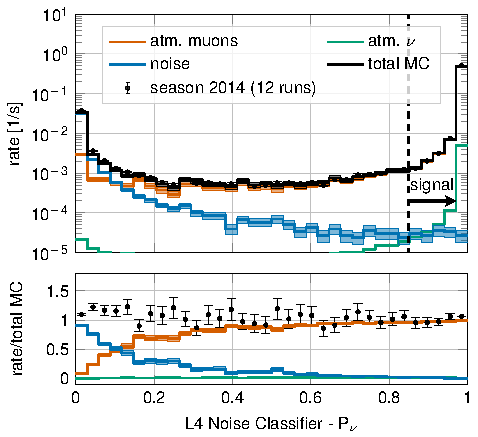
\includegraphics[width=0.49\linewidth]{figures/simulation_and_processing/selection/l4_noise_classifier_probnu.pdf}
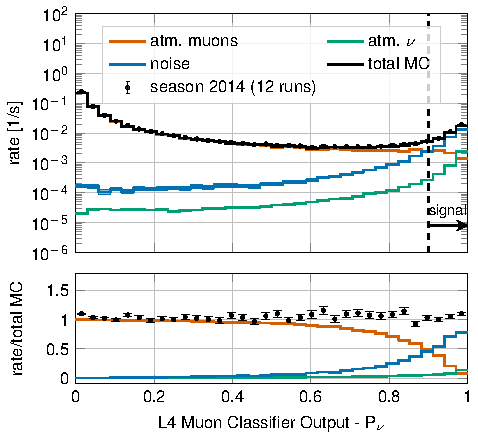
\includegraphics[width=0.49\linewidth]{figures/simulation_and_processing/selection/l4_muon_classifier_probnu.pdf}

\caption[Level 4 classifier outputs (muon and noise)]{Distributions of Level 4 noise classifier output (left) and muon classifier output (right), where larger values indicate more neutrino-like and lower values more noise-like/. Taken from \cite{OVS_PRD}.}
\labfig{level_4_classifiers}
\end{figure*}


\subsubsection{Level 5} \labsec{level_5}

Level 5 is the final selection level, before event reconstructions are applied. This level aims to reduce the remaining atmospheric muon rate below the rate of neutrinos. Muons not rejected by the earlier levels are those that produced little or no light in the veto regions. One possible reason is that they passed through one of the un-instrumented regions between the strings \todo{add some figure showing the corridors?} called \textit{corridors}. To reject those, special corridor cuts, based on the number of hits they produced close to a potential corridor they passed through. The potential corridor in questions is identified based on a simple infinite track fit. In addition to the corridor cuts, starting containment cuts are applied to reject events that start at the edge of the fiducial volume. Events with more than seven hits in the outermost strings of the detector or those that have a down going direction in the uppermost region are rejected. This further reduces the fraction of muons by \SI{96}{\percent} while keeping \SI{48}{\percent} of neutrinos. The rates after this level are \SI{1}{\milli\hertz} and \SI{2}{\milli\hertz} for neutrinos and muons, respectively, making it a neutrino dominated sample.

\todo{add table with rater per level (split in flavor for signal (benchmark mass/mixing?) and background)}


\section{Reconstruction} \labsec{reconstruction}

Several methods exist to reconstruct events at the energies relevant for this work (\SIrange{10}{100}{\gev}). At these energies, the light deposition is very low and only a few DOMs detect light, making the reconstructions difficult. \sidecite{low_energy_reco_IC} describes two classical methods, which have partly been applied in one recent IceCube atmospheric neutrino oscillation measurement using a
% golden\sidenote{The golden sub-sample only uses events that have direct photon hits.} 
sub-sample of the DeepCore sample \sidecite{OVS_PRD}. The algorithm used in this work on the other hand, is a newer method that applies a \textit{convolutional neural network (CNN)} to reconstruct the events and determine some discriminating quantities. The latest muon neutrino disappearance result from IceCube \sidecite{flercnn_analysis_result} is based on this reconstruction.


\subsection{Fast Low Energy Reconstruction using Convolutional Neural Networks} \labsec{flercnn_reconstruction}

As the name \textit{Fast Low Energy Reconstruction using Convolutional Neural Networks (FLERCNN)} already indicates, the FLERCNN reconstruction \sidecite{flercnn_proceedings, flercnn} is a CNN optimized to reconstruct IceCube events at low energies ($<$\SI{100}{\gev}) in a fast and efficient manner. The network is trained to find the connection between the hit pattern and the events properties by identifying patterns similar to how CNNs are applied effectively in image classification.\todo{add references for CNN image classification?} The patterns are an imprint of the neutrino interactions that can happen anywhere in the detector, which should result in translational invariance of the events. CNNs were shown to have very good performance in identifying patterns in images, independent of their location. By combining several layers of filters of different dimensions, a map of spatial features is created from the input data and more complex features can be reconstructed. The architecture of the network is very similar to the preexisting IceCube CNN event reconstruction \sidecite{dnn_reco_mirco}, but optimized on low energy events and specifically tailored to include the DeepCore sub-array. Only the eight DeepCore strings and the central 19 IceCube strings are used for the reconstruction (compare to \reffig{icecube_top_view}). Because of the different z-positions of the DeepCore and IceCube DOMs, they are divided into two networks that are combined at the end. The full architecture is shown in \reffig{flercnn_network_structure}. The first dimension of the network is the string index, while the second dimension is the order of the DOMs along the vertical axis. The horizontal position of the DOMs is not used, since the strings are arranged in an irregular pattern. The information from the DOM hits is summarized into five charge and time variables, which make up the last dimension of the input layer. The variables are the total summed charge, the time of the first hit, the charge weighted mean time of the hits, the time of the last hit, and the charge weighted standard deviation of the hit times.

\todo{add image with selected strings used for flernn IC and DC}

\begin{figure}
    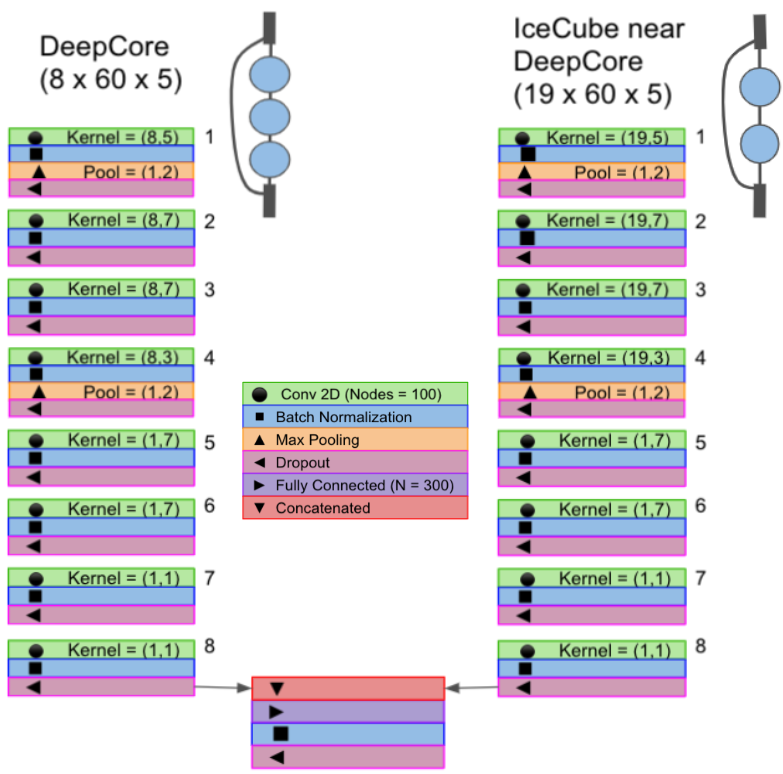
\includegraphics{figures/simulation_and_processing/flercnn/Detailed_CNN_Architecture_combined.png}
	\caption[FLERCNN architecture]{Architecture of the FLERCNN neural networks, taken from \cite{flercnn_proceedings}.}
    \labfig{flercnn_network_structure}
\end{figure}


Five different networks are trained using this architecture. Three networks do the regression of the events' energy, zenith angle, and the starting vertex ($x,y,z$ position), while two of them are used for classification. One to predict the probability of the event being a track (used as PID) and the other to predict the probability of the event being a muon. Each network is trained with a modified training sample, optimized for the task it is performing, but unbiased for the training variable and ideally extending outside the target reconstruction region. Additionally, the activation function and the loss function are adapted, according to the wanted output of the network. For the classification tasks the loss function is the \textit{binary cross entropy} and the activation function is a \textit{sigmoid}. To perform the regression of zenith and vertex position, the loss function is the \textit{mean squared error (MSE)}, while for the energy it is the \textit{mean absolute percentage error}. The activation for all regression tasks is \textit{linear}.

\todo{add some performance plots of the FLERCNN reconstruction}

\todo{There is more information on pre-processing the samples and preparing the input features, and training each cnn, but I'm not sure if that might be too much detail?}

% \textit{INFO on resolutions:} Note that all analysis cuts are included in these resolution calculations, which results in an artificial resolution decrease near $E_{true} \approx 100$ GeV in Figure \ref{fig:EnergyResolution} due to the cut at $E_{reco} < 100$ GeV.


\subsection{Analysis Selection} \labsec{analysis_cuts}

Before the reconstruction is applied a few additional high level variables are computed, which are from fast and inexpensive algorithms. Then the reconstruction is performed by applying the trained FLERCNN networks to get the output quantities. After that, another BDT classifier is trained to further reduce the muon background for the final sample. The BDT is trained on five high level variables, where three are FLERCNN reconstruction variables (vertex $z$, $\rho_{36}$\sidenote{A radial variable that is often used in IceCube, is the horizontal distance to string 36 called $\rho_{36}$, which is basically the distance to the center of IceCube.}, and muon probability) and two are lower level variables (L4 muon classifier output and L5 corridor cut variable). To train the BDT, the FLERCNN nominal simulation set is used, only using events with $\cos(\theta_{zenith})\leq 0.3$. The output of the BDT is the neutrino probability and a cut at 0.8 is applied to reject events with a high probability of being a muon. \reffig{muon_bdt_id} shows the output of the BDT classifier, where the neutrinos in both training and testing sets are gathered at 1 and muons are around 0, which shows great classification power.

\begin{figure*}
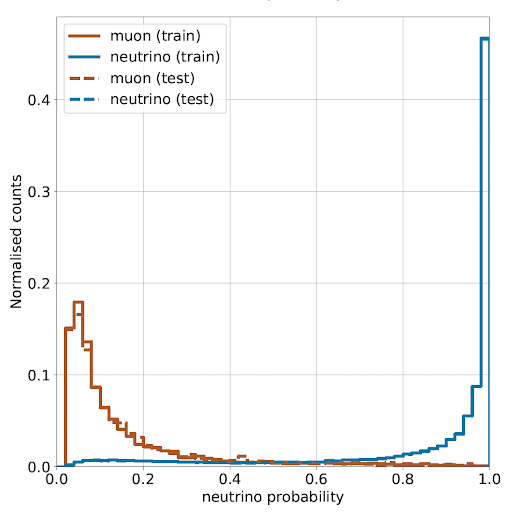
\includegraphics[width=0.49\linewidth]{figures/simulation_and_processing/flercnn/flercnn_muon_classifier.png}
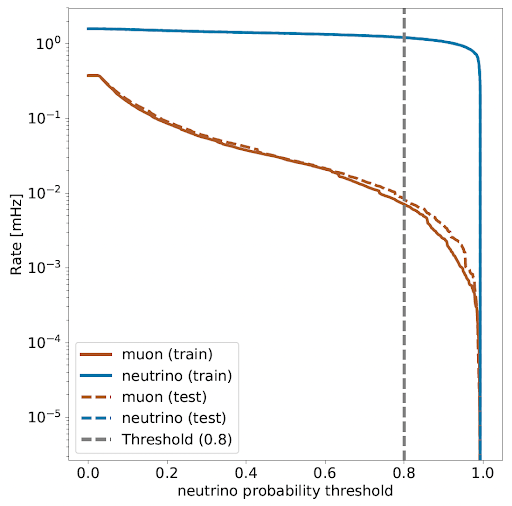
\includegraphics[width=0.49\linewidth]{figures/simulation_and_processing/flercnn/flercnn_muon_classifier_rate_vs_threshold.png}
\caption[FLERCNN muon classifier probability distributions]{FLERCNN muon classifier output score (left) and rate of neutrinos and muons as function of muon classifier cut (right). Taken from \cite{flercnn_analysis_internal_note}}
\labfig{muon_bdt_id}
\end{figure*}

\todo{add reference for flercnn analysis internal note}

To get the final, pure sample of well reconstructed neutrinos another set of cuts is applied. The first cuts are meant to reject events with poor reconstruction quality, by requiring the events to fall into the DeepCore volume, where the denser, better instrumented detector leads to better resolution. The cuts are applied on the vertex $z$ and $\rho_{36}$ and are listed in \reftab{analysis_cuts}. The FLERCNN reconstruction was optimized for atmospheric neutrino analyses which are mainly in the region below \SI{100}{\gev} and there are very few events with energies below \SI{5}{\gev}, so the reconstructed energy is required to be in that range. Additionally, rejecting events with fewer than seven hits in the selected DOMs used for FLERCNN showed to increase the resolution.

Another set of cuts is applied to make sure the agreement between data and MC is good. To remove coincident muon and neutrino events, cuts are applied to the number of hits in the top 15 layers of IceCube DOMs and the number of hits in the outermost IceCube strings. Coincident random noise events are removed by requiring more than three hit DOMs from direct photons\sidenote{\textit{Direct photons} are photons that were not scattered on their way from the interaction vertex to the DOM.}. Neither of the two coincident event types are simulated, which can be seen as bad agreement between data and MC. The last cut is on the reconstructed cosine zenith, which is required to be smaller than 0.04 to reject down-going muons.

\begin{table}
    \small
        % \begin{tabular}{ p{0.36\textwidth} p{0.26\textwidth} p{0.25\textwidth} }
        \begin{tabular}{ lll }
        \hline\hline
    
        \textbf{Variable} & \textbf{Threshold} & \textbf{Removed} \\ 
    
        \hline\hline
    
        Number of hit DOMs & $\geq 7$ & \SI{1.05}{\percent} \\
        Radial distance & < \SI{200}{\meter} & \SI{0.09}{\percent} \\
        Vertical position & \SI{-495}{\meter} < z < \SI{-225}{\meter} & \SI{5.48}{\percent} \\
        Energy & \SI{5}{\gev} < E < \SI{100}{\gev} & \SI{20.70}{\percent} \\
    
        Cosine of zenith angle & < 0.04 & \SI{19.66}{\percent} \\
        Number of direct hits & > 2.5 & \SI{10.50}{\percent} \\
        Number of hits in top layers & < 0.5 & \SI{0.03}{\percent} \\
        Number of hits in outer layer & < 7.5 & \SI{0.001}{\percent} \\
        Muon classifier score & $\geq 0.8$ & \SI{23.90}{\percent} \\

        \hline
        \end{tabular}
    \caption[Final analysis cuts]{Cuts performed to select the final analysis sample. Parts of the cuts are meant to increase the data/MC agreement, while others are meant to reject events with poor reconstruction quality.}
    \labtab{analysis_cuts}
    \end{table}
    

\todo{there is some more information in Elisas thesis about the  final sample composition, but I should maybe put this together for myself?}

\todo{at some place I will want a selection efficiency plot for SM BG and HNL signal, but I'm not sure where to put it yet}


\section{Systematic Uncertainties} \labsec{systematic_uncertainties}

There are multiple sources of systematic uncertainties related to the event generation and processing explained in this chapter. Since variations in the range of these uncertainties change the expected number of events in the analysis, it is important to estimate their impact on the final results. In this work the aim is to be able to continuously vary the systematic parameters, modeling their effects, so that a simultaneous fit of the physics and systematic parameters can be performed. Where possible, a correct model of the effect is used, but in many cases the variations are captured by effective parameters. Uncertainties that solely scale the total event rate are not included individually, since the analysis only uses the relative distribution of events. A single scaling parameter $A_\rm{eff}$ is used to scale the total neutrino rate instead.


\subsection{Atmospheric Flux Uncertainties}

The flux of atmospheric neutrinos is influenced by multiple factors, the spectrum and composition of cosmic rays, the assumed atmospheric conditions, and the hadronic interaction model used to describe the air showers development. Uncertainties of the neutrino flux are therefore dictated by the uncertainties on these components, where the variations in atmospheric conditions were found to have negligible effect \sidecite{OVS_PRD}.


\paragraph{Cosmic ray flux:}

The selected sample of atmospheric neutrinos lies around energies of up to \SI{100}{\gev}. The initial primary particles in the cosmic ray flux can have 100 times larger energies and therefore the cosmic ray flux between \SI{10}{\gev} and \SI{10}{\tera\electronvolt} is important, which dominantly consists of helium and proton \sidecite{cosmic_ray_composition_and_GSF}. The uncertainty in this cosmic ray flux component can be described as a power law correction \sidecite{PhysRevD.74.094009, PhysRevD.95.023012}
\begin{equation}
    \Phi^\prime_\nu = \Phi_\nu \left( \frac{E}{E^\star} \right)^{\Delta\gamma}
    \;,
    \labeq{power_law_flux_uncertainty}
\end{equation}
where $E^\star$ is the pivot energy and $\Delta\gamma$ is the correction to the power law exponent. This modification propagates into the neutrino flux, which is therefore corrected in the same way. $E^\star$ was chosen to be \SI{24}{\gev} as to minimize the dependence of the overall flux scale on $\Delta\gamma$ \sidecite{OVS_PRD}.


\paragraph{Hadronic interaction model:}

Neutrinos are produced in the decaying hadrons in cosmic ray air showers, spanning a large parameter space that is sparsely evaluated by experimental data. To include uncertainties based on energy, direction, and neutrino flavor, the \textsc{MCEq} package \sidecite{mceq} is used to compute the distribution of atmospheric leptons and to estimate the impact of varying their contributions. The calculations in MCEq are based on the work of Barr \textit{et al.} \sidecite{Barr:2006it} and results in the change in flux $d\Phi_\rm{l}/dB$ for a variation $dB$ of some parameter $B$. Scaling this variation by some value $b$, the modified total flux, s is then given by
\begin{equation}
    \Phi^\prime_\rm{l} = \Phi_\rm{l} + \left( b \cdot \frac{d\Phi_\rm{l}}{dB} \right)
    \;.
    \labeq{mceq_flux_variations}
\end{equation}
Matching the original work, the parameter space is divided in the primary energy $E_i$ and the energy fraction of the secondary meson $x_\rm{lab}$, with varying uncertainties, derived from fixed target experiment data. The Sibyll2.3c \sidecite{sibyll2.3d} hadronic interaction model and the GSF cosmic ray flux \sidecite{cosmic_ray_composition_and_GSF} were used to calculate the related flux changes\sidenote{The choice of flux and hadronic interaction model have minor impact on the variations.} for the different regions in $E_i$ and $x_\rm{lab}$, resulting in 17 variables, encoding the possible changes.


\subsection{Cross-Section Uncertainties}

The uncertainties related to the cross-sections are split into low and high energy components, since there is no coherent model to explain both DIS interactions, which are the dominant processes above \SI{20}{\gev}, and \textit{charged current resonance production (CCRES)} and \textit{charged current quasi elastic scattering {CCQE}}, which are relevant below \SI{20}{\gev} where interactions with the nucleons as a whole are important. Three parameters are included to account for all relevant cross-sections uncertainties.

At low energies two parameters are included accounting for uncertainties in form factors of CCQE and CCRES events. These uncertainties are due to uncertainties in the \textit{axial mass} $M_\rm{A}$, which enters the form factor as in
\begin{equation}
    F(Q^2) \sim \frac{1}{(1 - (\frac{Q}{M_\rm{A}})^2)^2}
    \;,
\end{equation}
where $Q^2$ is the momentum transfer squared. The axial mass can be determined experimentally\todo{which experiments measure the axial mass?} and to include uncertainties on the values of $M_\rm{A}^\rm{CCQE}$ and $M_\rm{A}^\rm{CCRES}$, the cross-sections are computed with GENIE, where the form factors are calculated varying the axial mass by $\pm 20\% (1\sigma)$/$\pm 40\% (1\sigma)$ around the nominal value. This is an approximation of the recommended uncertainties by the GENIE collaboration, which are $-15\%$, $+25\%$ for $M_\rm{A}^\rm{CCQE}$ and $\pm 20\%$ for $M_\rm{A}^\rm{CCRES}$ \cite{genie}. To apply a continuous uncertainty variation of the axial mass in a fit, the total cross-section is fit with a quadratic function to interpolate between the cross-sections computed with the different axial masses.

Even though the DIS interactions can be calculated very precisely, there are still uncertainties in the input PDF, describing the probability of finding a specific parton (quark) with a specific momentum fraction $x$ inside a nucleon. To account for differences between the used method and more sophisticated methods using newer PDFs seen at high energies, an uncertainty parameter is introduced. The parameter is based on the discrepancy between the cross-sections computed with GENIE and the ones computed with CSMS \sidecite{csms} above \SI{100}{\gev}. The included parameter scales the cross-section from the GENIE values to the CSMS values, which are considered more accurate above \SI{100}{\gev}. The scaling is done as a function of energy and inelasticity and to guarantee continuity, the scaling is extrapolated linearly below \SI{100}{\gev}. The parameter is designed such that a value of 0.0 corresponds to the GENIE cross-sections and a value of 1.0 gives an approximation of the CSMS cross-sections. A comparison of the total cross-sections GENIE (scaled/unscaled) with the data is shown in \reffig{dis_systematic_effect}.

\begin{figure*}
    \centering 
    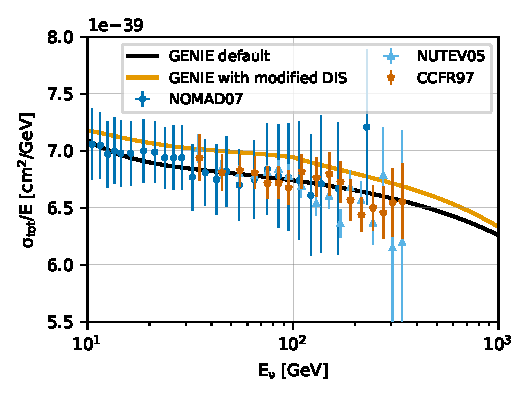
\includegraphics[width=0.49\linewidth]{figures/simulation_and_processing/cross_sections/NuMu_CC_iso_comp_to_data__upd_style.pdf}
    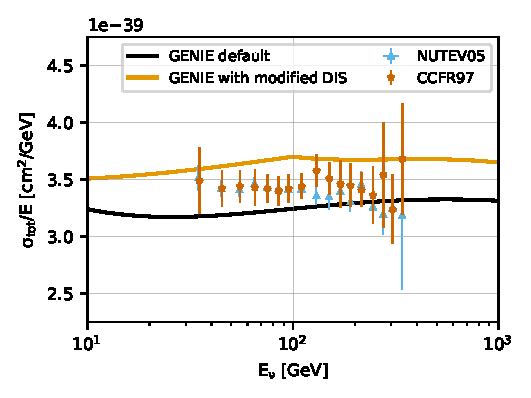
\includegraphics[width=0.49\linewidth]{figures/simulation_and_processing/cross_sections/NuMu_Bar_CC_iso_comp_to_data__upd_style.pdf}
    
    \caption[Inclusive total neutrino-nucleon cross-sections]{Inclusive total neutrino-nucleon cross-sections on an isoscalar target (black) for neutrinos (left) and antineutrinos (right) calculated with GENIE, comparing to measurements from NOMAD \cite{xsec_data_nomad}, NUTEV \cite{xsec_data_nutev}, and CCFR \cite{xsec_data_ccfr}. The scaled GENIE cross-section (orange) is also shown. Taken from \cite{OVS_PRD}.}
    \labfig{dis_systematic_effect}
\end{figure*}


\subsection{Detector Calibration Uncertainties}

There are multiple sources of systematic uncertainties related to the detection process of neutrinos in IceCube. Dominant for this analysis are the effects of the properties of the ice itself and the optical efficiency of the DOMs. None of these uncertainties can be described by an analytic expression, so they have to be estimated using MC simulation. The method used to derive the continuous variations based on the MC simulation is described in \refsec{ultrasurfaces}. The five relevant uncertainty parameters are the absolute efficiency of the DOMs, a global scaling of bulk ice scattering and absorption lengths, and variations of the relative angular acceptance in two parameters.


\paragraph{DOM efficiency:}
As was already mentioned in \refsec{ice_and_DOMs}, the absolute efficiency of the DOMs is calibrated using minimum ionizing muons from air showers, due to the lack of a calibrated light source in the detector. Using the muons as a steady, controlled source of light, the efficiency can be estimated by comparing simulated muon data sets with varied DOM response to the measured data. Since the uncertainties found in multiple iterations of this study \sidecite{JFeintzeig_phd, domeff_nick} are at the order of \SI{10}{\percent}, this systematic is highly relevant and has to be included in the analysis.


\paragraph{Bulk ice scattering and absorption:}



\paragraph{Hole ice angular acceptance:}




\subsection{Muon Uncertainties}

The muon fraction in the final level selection (see \refsec{analysis_cuts}) is below \SI{1}{\percent}, therefore additional muon systematic uncertainties apart from the spectral index are not implemented, but rather a total muon scaling parameter is added. This total scale is somewhat degenerate with the DOM efficiency, since an increased DOM efficiency leads to better muon rejection\todo{cite this?}. Both the total muon scaling and the muon spectral index have a very small impact on the analysis as will be shown in \refsec{parameter_selection}.
